\documentclass{article}
\usepackage{titlesec}
\usepackage[parfill]{parskip}
\usepackage[utf8]{inputenc}
\usepackage{cite}
\usepackage{amsmath}
\usepackage{graphicx}

\title{\textbf{Headlights}: \\
Training the next generation to \\
better predict the future.}
\author{William Henderson and Dron Hazra \\
\\
\textit{HackX $\cdot$ University of Cambridge}
}
\date{November 2022}

\titlespacing*{\subsection}{0pt}{5mm}{2mm}

\begin{document}

\maketitle

\section{Abstract}

Existential threats to humanity can only be mitigated if they can be predicted. Statistical models, such as those used in climate science, have been used since the 1960s \cite{noaa}, but they have their limitations. Human intuition, when combined with statistical modelling, can improve predictions, as demonstrated by superforecasters \cite{superforecasters}. In this paper, we present a novel approach to training this aspect of human intuition using historical data in a game-like environment.

\section{Introduction}

A superforecaster is a person who is able to make accurate predictions about the future. Superforcasters' predictions have had a great impact on the world, for example during the COVID-19 pandemic, in which their ``eerily accurate'' predictions were frequently correct, despite often going against those of governments \cite{covid19}. However, superforecasters are few and far between, so a method of training more people to make accurate predictions of the future is needed.

Conventional approaches to training superforecasters include using tools like Metaculus \cite{metaculus}, which is a website that crowdsources predictions about current events and rewards those whose predictions are accurate. These tools are very powerful, but the feedback loop is long - it can take weeks or months for a prediction to be resolved - so it takes a long time to improve.

We propose a novel approach called Headlights, which uses a game-like environment to train people based on historical data. Instead of using current events, Headlights presents users with several years of historical data, and asks them to predict some variable a few years after the end of the data. The application also provides a limited search engine, which returns only data and newspaper articles from the period of the data. This allows users to gain an insight into the historical context of the data, and to use this context to make predictions, just as is done in the present day.

\section{Methods}

A user is presented with a graph of historical data, spanning anywhere between 10 and 20 years. The user is then asked to predict some variable a few years after the last data point, with the help of other data and newspaper articles from the period. The user's response is given as a range of values, and the application then calculates the user's score based on the accuracy of their prediction, a process called ``calibration''.

This process can be repeated as many times as the user wishes, and the application keeps track of the user's score. Since there is no need to wait for a prediction to be resolved, this allows the user to improve their ability to predict the future much faster than with existing tools.

\subsection{Calibration}

Calibration measures the validity of probability assessments. It is a measure of how well a user's predictions match the actual outcome \cite{calibration}. It would be unreasonable and unrealistic to ask the user for an exact value, so instead the user is asked to provide a range of values corresponding to their 90\% confidence interval. The user's score is then calculated based on how often the outcome falls within their predictions.

If 90\% of the user's predictions are correct, then the user is said to be calibrated and this gives them the greatest score. If the user gets more right than this, then they are underconfident, which means that their intervals are too wide and hence their score is reduced. Conversely, if the user gets less right than this, then they are overconfident, which means that their intervals are too narrow and likewise they are penalised.

The scoring function is given by:

$$
S(c, n) = \dfrac{
  \binom{n}{c} \cdot 0.9^c \cdot 0.1^{n-c}
}{
  \binom{n}{0.9n} \cdot 0.9^{0.9n} \cdot 0.1^{0.1n}
}
$$

where $c$ is the number of correct predictions in $n$ predictions. This function is analagous to the binomial distribution, normalised so that the maximum score is 1 (i.e. the user is calibrated).

\subsection{Sourcing Data}

A platform like Headlights requires a huge amount of datasets to be useful. Much of this data can be retrieved from aggregators like Our World in Data \cite{ourworldindata}, alongside primary sources such as the US Government's data portal Data.gov.

Headlights also provides access to important historical newspaper articles, which were retrieved from the BBC's On This Day archive \cite{onthisday}. They span the period from 1950 to 2005, with between 10 and 20 of the most significant articles from each year.

\subsection{Interface}

The interface is designed to be as simple and intuitive as possible, to allow the user to focus on the data. The user has access to a search bar, which returns data and articles from the period of the data they are analysing. Figure \ref{fig:interface} shows the interface.

\begin{figure}[h]
  \centering
  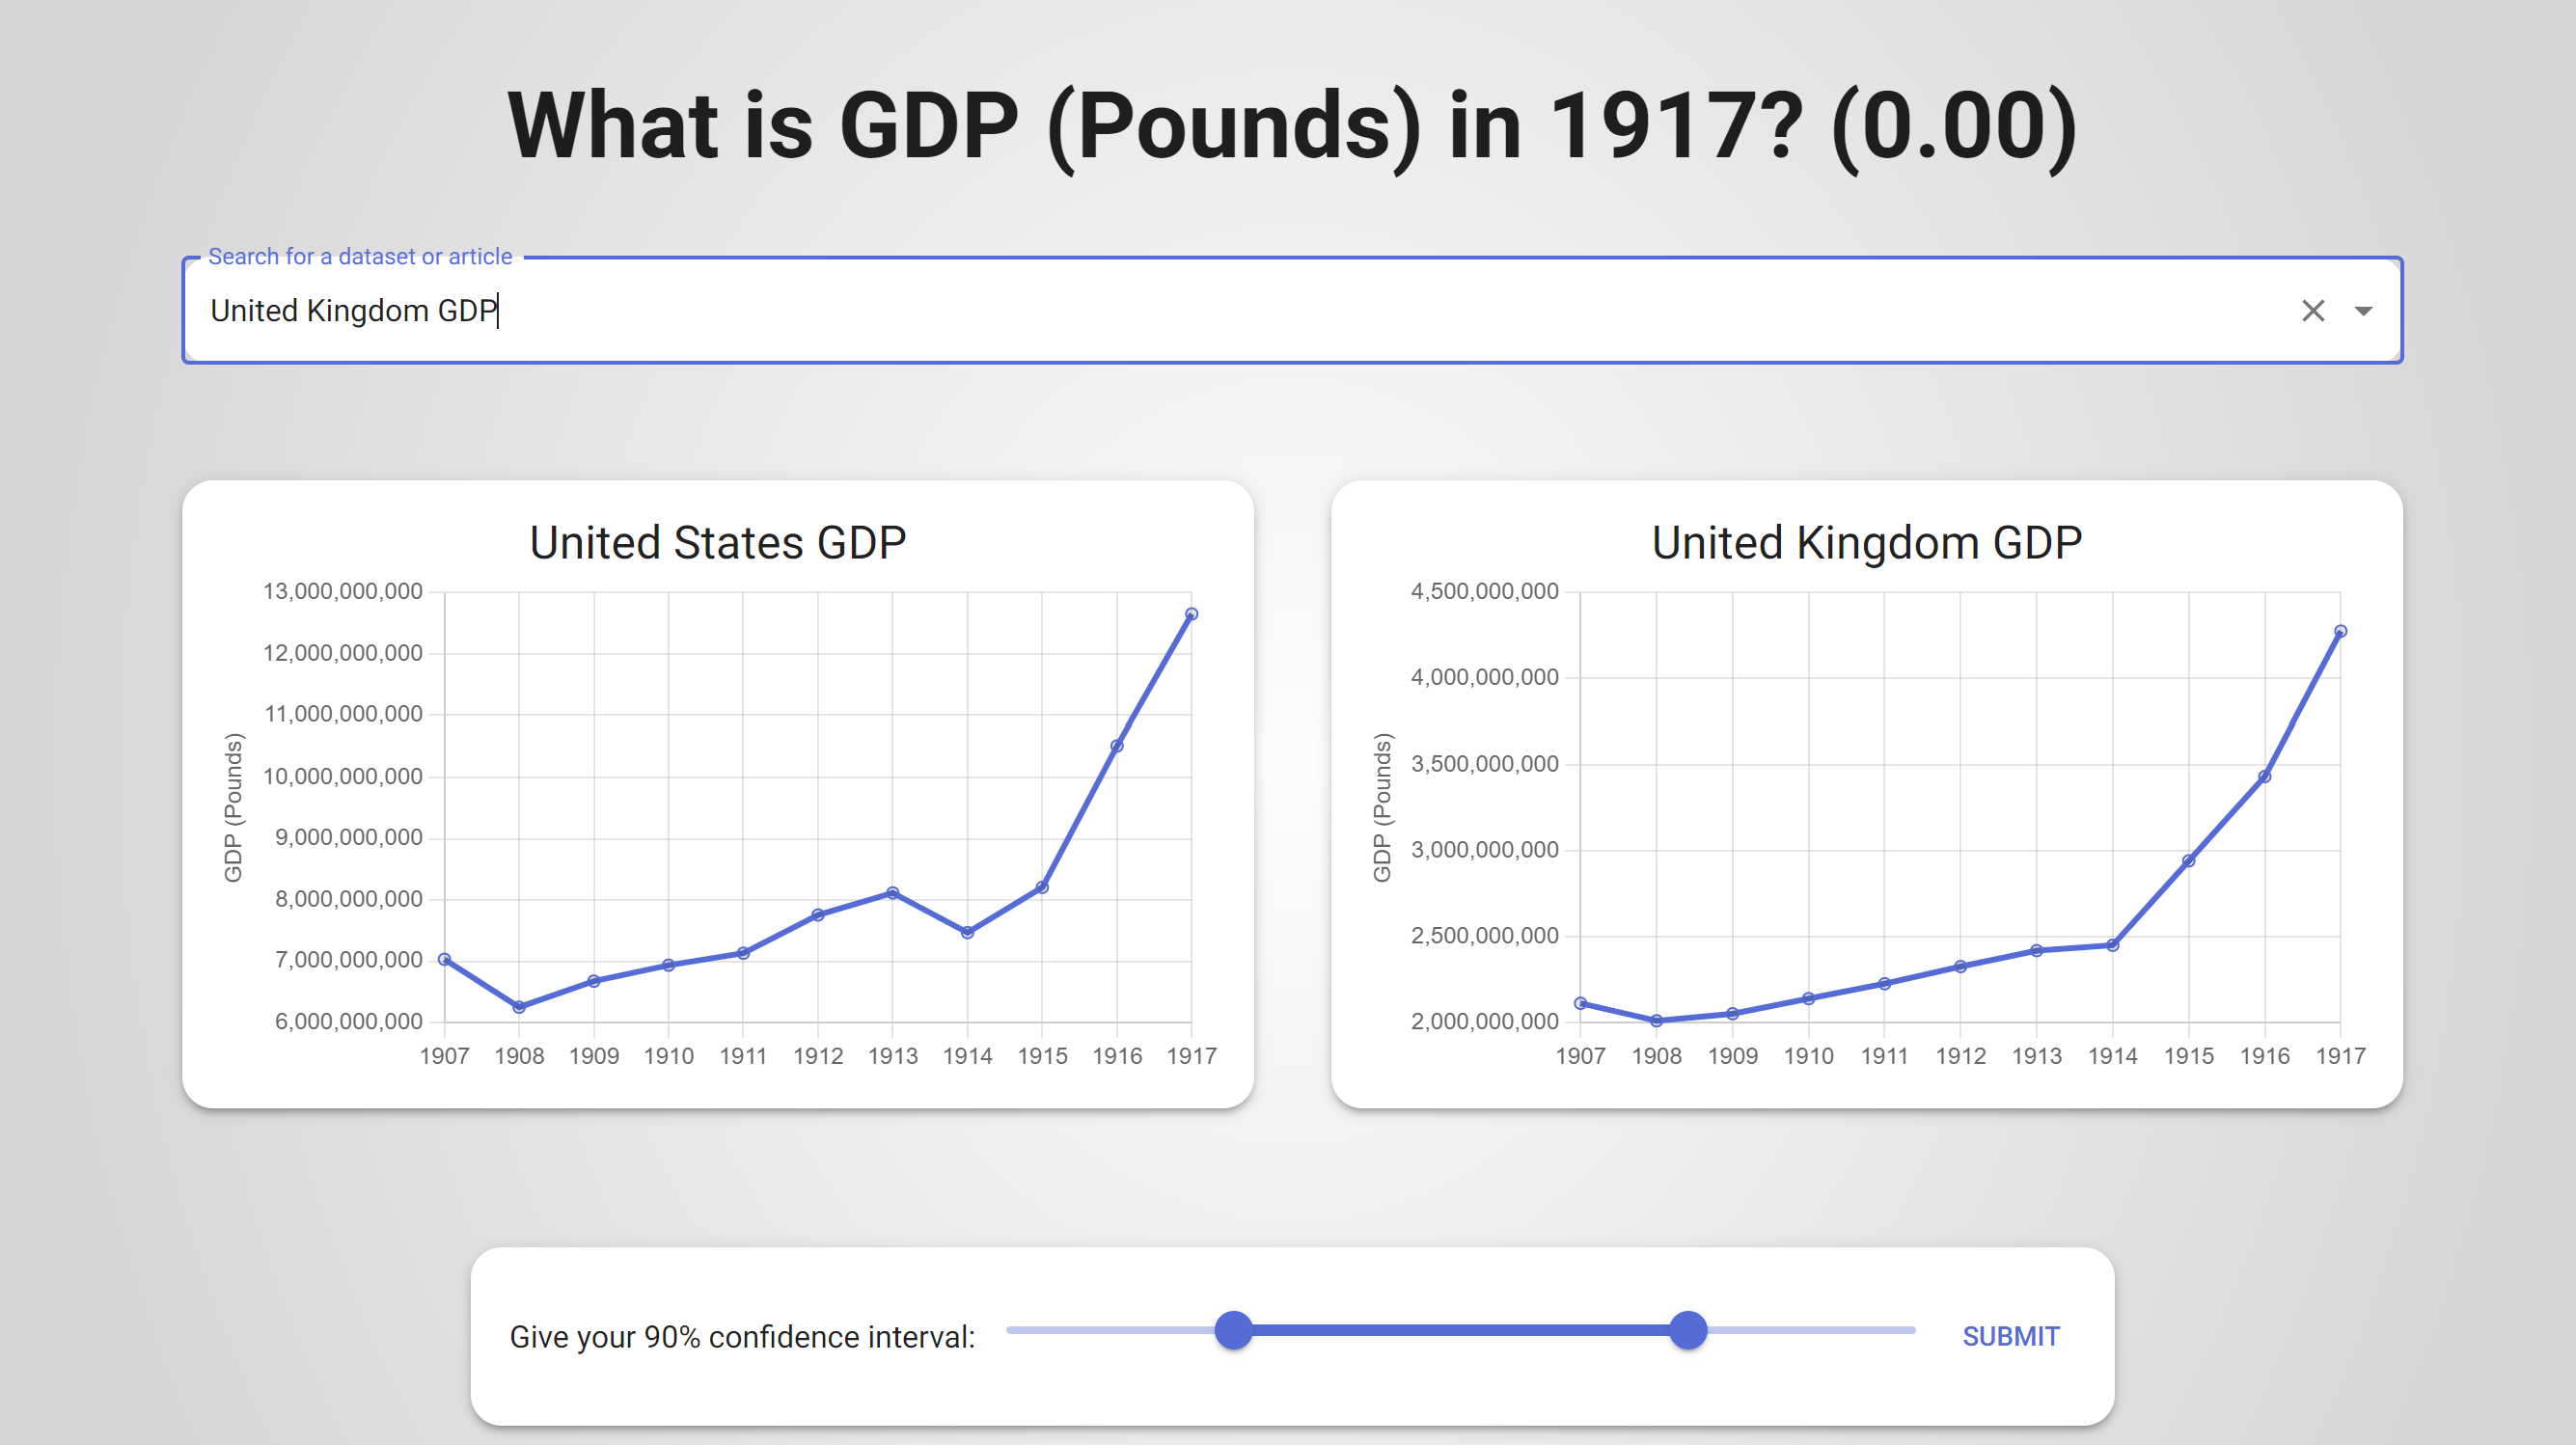
\includegraphics[width=\textwidth]{screenshot.png}
  \caption{Screenshot of the Headlights application.}
  \label{fig:screenshot}
\end{figure}

\newpage

\subsection{Architecture}

The application uses a React frontend, which communicates with a Rust backend. The frontend is responsible for displaying the data and articles, as well as for the scoring and calibration functions. The backend is responsible for retrieving, filtering, and manipulating the data and articles from a variety of sources.

Figure \ref{fig:architecture} shows this architecture.

\begin{figure}[h]
  \centering
  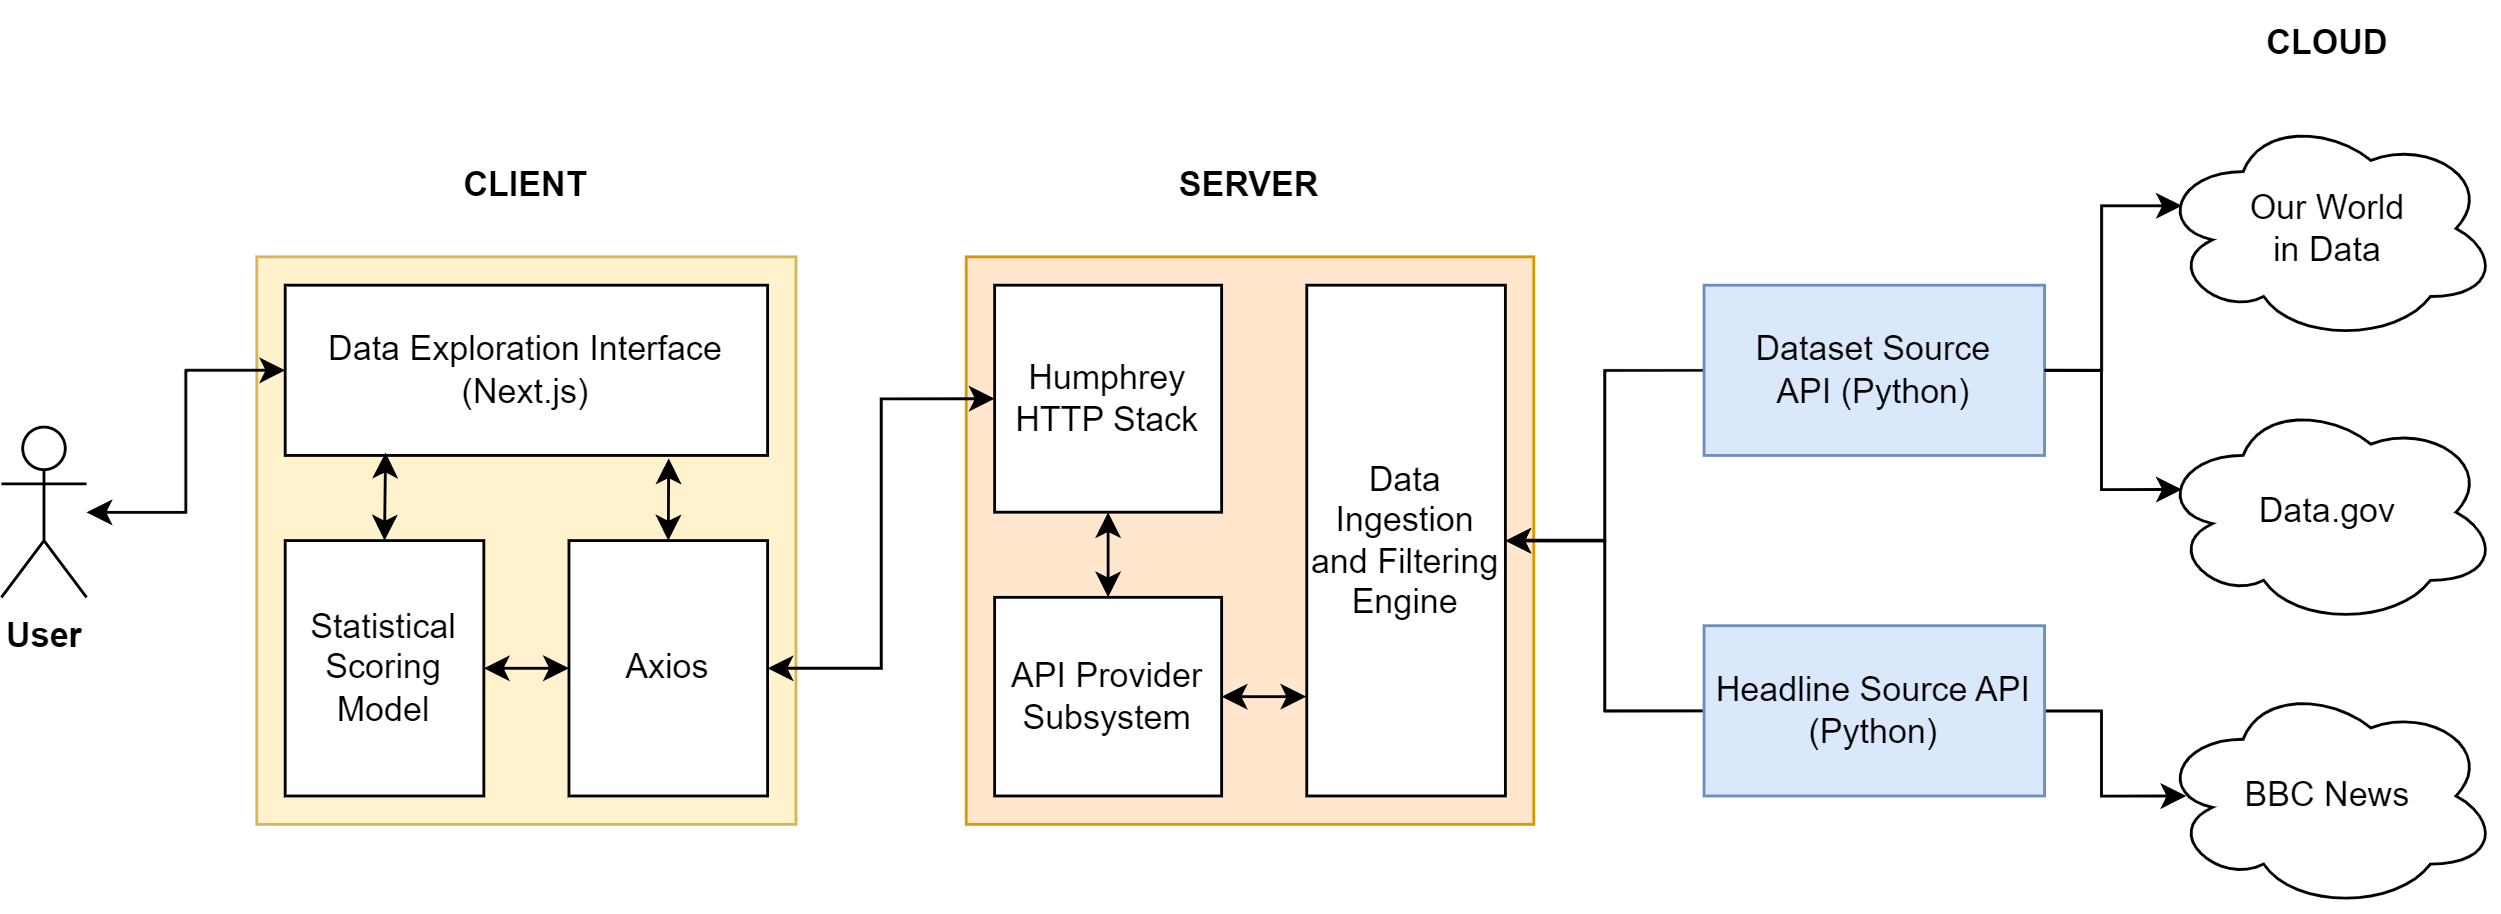
\includegraphics[width=\textwidth]{architecture.png}
  \caption{Architecture of the Headlights application.}
  \label{fig:architecture}
\end{figure}

\section{Discussion}

A key issue with this approach is that using historical data may introduce bias. For example, if the user is given life expectancy data for the UK from 1900 to 1910, and asked to predict life expectancy in 1915, then their prediction may be unconsciously influenced by prior knowledge about the First World War. This problem can be mitigated by using a large number of varied datasets from around the world, in the hope that the user's general historical knowledge will not be broad enough to make a significant contribution to their predictions.

Another issue is that of whether the user can improve their predictions enough to be useful. This was not something we were able to test due to time constraints, but we believe that the approach is promising enough to warrant further research.

\subsection{Theory of Change}

The ultimate goal of Headlights is to help prevent existential threats to humanity. However, to prevent these threats we need to predict them. This is a difficult task, and one that can be approached using statistics, machine learning, human intuition, or a combination of these. In order for human intuition to be able to accurately make these predictions, it needs to be trained and improved. Headlights is designed to do this while also providing statistical data and historical context as would be the case in the real world.

\section{Conclusion}

We have presented a novel approach to training people to make more accurate predictions about the future. This approach uses historical data and newspaper articles to provide context for the user's predictions, and uses a fast-paced gamified environment to allow the user to quickly improve. We believe that this approach has the potential to be a useful tool for training people to make better predictions, and these predictions could be vital in predicting and mitigating existential risks.

\bibliography{refs}{}
\bibliographystyle{unsrt}

\end{document}